% Chapter Template

\chapter{Sistema de monitoratge} % Main chapter title

\label{SistemaMonitoratge} % Change X to a consecutive number; for referencing this chapter elsewhere, use \ref{ChapterX}

En aquest punt tenim la base necessària per procedir a exposar el treball realitzat des d'un punt de vista de disseny software i implementació dels diferents components. Agafant com a referència la solució proposada al \textit{Capítol 5. Visió general del sistema}, procedirem a desenvolupar els detalls tècnics de cadascun dels components que integren aquest sistema. Començarem per explicar els detalls relacionats amb el disseny i la implementació dels monitors.

\section{Monitors}

Recordem que, dins el nostre context, un \textbf{monitor} consisteix en un \textbf{component software} autònom amb una activitat regular orientada al control de qualitat d'un altre sistema software. Aquest control de qualitat es basa en una col·lecció de dades obtingudes a través d'aquest segon sistema, que ens aporten informació pròpia del context monitorat. Amb aquestes dades, un sistema capacitat per processar i analitzar aquestes dades, es poden generar suggerències de modificacions. Aquesta darrera part, però, queda fora de l'abast del nostre projecte, que centrarà l'activitat dels monitors en la seva tasca principal: la col·lecció de dades sota una sèrie de criteris específics.\\

En general, per tant, volem que el nostre sistema disposi d'un conjunt de monitors heterogenis (i, per tant, de naturalesa i comportament diferents), que puguin ser capaços de gestionar \textbf{processos de monitoratge} de forma paral·lela. És a dir: cadascun d'aquests monitors ha de ser capaç d'inicialitzar processos de monitoratge que s'executin en paral·lel i en segon pla, col·lectin dades d'acord als criteris de cadascun d'aquests processos, i les redireccionin a un tercer component software, encarregat del seu anàlisi.Per tant, necessitem que cadascun d'aquests monitors satisfaci els següents requisits funcionals:

\begin{enumerate}
\item \textbf{Inicialització de procés de monitoratge.} El monitor ha de poder rebre una petició per inicialitzar un nou procés de monitoratge amb una sèrie de paràmetres de configuració que defineixin aquest procés de monitoratge.
\item \textbf{Modificació de procés de monitoratge.} Donat un procés de monitoratge ja existent, el sistema ha de permetre la seva reconfiguració. És a dir: el sistema ha de permetre modificar els paràmetres d'aquest procés i, en conseqüència, alterar el comportament del procés (d'acord amb els criteris que es presenten a continuació.
\item \textbf{Aturada de procés de monitoratge.} Donat un procés de monitoratge ja existent, el sistema ha de permetre la seva aturada. Davant aquesta petició, el procés s'atura, i per tant es deixen de recol·lectar dades sota aquells criteris de monitoratge.
\end{enumerate}

\subsection{Especificacions tècniques i funcionals}

Tal i com establiem com a objectiu principal del projecte, aquest sistema de monitoratge ha de ser \textbf{heterogeni}. La conseqüència principal d'aquesta característica és que necessitem definir un sistema que contempli que cadascun d'aquests requisits funcionals es garanteixen en la integració dels monitors implementats, i que per tant esdevenen casos d'ús complets i satisfactoris del nostre context. Per fer-ho, i donat que els monitors seran el principal punt de variabilitat del nostre sistema, hem d'afegir un cert nivell d'abstracció, un \textbf{desacoblament} entre els detalls específics de cadascun dels monitors, que ens resulten indiferents per la resta del sistema.\\

Per tant, el primer pas que hem de realitzar és \textbf{dissenyar una arquitectura} i uns \textbf{criteris de configuració genèrics} que satisfacin dos criteris: primerament, que ens permetin integrar tots els monitors implementats sota aquesta proposta al nostre sistema; i en segon lloc, que permetin una independència suficient com per garantir el criteri d'heterogeneïtat dels monitors. Desenvoluparem aquesta proposta analitzant els següents punts:

\begin{enumerate}
\item \textbf{Comportament intern del monitor.} Anàlisi de les necessitats i detalls tècnics del funcionament intern del procés de monitoratge.
\item \textbf{Redirecció de dades col·lectades.} Especificacions tècniques del mètode de gestió i redirecció de dades.
\item \textbf{Configuració dels monitors.} D'acord amb les necessitats anteriors, descriure quins paràmetres necessitarem per configurar els monitors.
\end{enumerate}

\noindent \textbf{\large Comportament intern del monitor}\\

\noindent La implementació d'un monitor representa, des d'un punt de vista semàntic, un component software encarregat de monitorar un component software concret. En aquest context específic, entendrem \textbf{monitorar} com la col·lecció periòdica d'un conjunt de dades produïdes de l'execució del sistema software monitorat. En base a aquesta definició, entendrem com a \textbf{procés de monitoratge} el cicle següent:

\begin{enumerate}
\item Inicialització de les estructures de col·lecció de dades
\item Captura de dades durant el transcurs d'un període de temps determinat
\item Enviament de les dades a un tercer component software
\end{enumerate}

Així, de forma periòdica, un procés de monitoratge recull durant un període de temps (o \textbf{\textit{time slot}}) específic totes les dades que el monitor ha estat configurat per recollir. Per tal que els monitors es puguin explotar al màxim, és imprescindible que aquests permetin l'\textbf{execució en paral·lel} de diversos processos de monitoratge, amb possibles diferències en els seus paràmetres de configuració (p.e., aquest \textit{time slot}).\\

Davant aquesta proposta, el comportament i potencial d'un monitor queda molt limitat, ja que elements com p.e. el mètode de recollida de dades, o fins i tot les dades recollides, queden molt limitats. En general, és molt possible que un sistema software pugui ser monitorat mitjançant diferents tècniques, com per exemple l'ús d'APIs, llibreries o components externs, etc. Per aquesta raó, si volem permetre que el nostre monitor ofereixi flexibilitat en aquest aspecte, hem de permetre l'ús de diferents eines, o \textbf{\textit{tools}}, que aquest monitor pot utilitzar indistintament per executar els processos de monitoratge.\\

La integració de diverses \textit{tools} dins un monitor ens permeten no només una variabilitat en l'execució de la col·lecció de dades, sinó també una major fiabilitat i qualitat del monitor com a component software. Ens permet reaccionar, entre d'altres, davant escenaris on l'ús d'un sistema de monitoratge específic deixa de funcionar (p.e. una API que no dona resposta), ja que davant la detecció d'aquest error el canvi de \textit{tool} utilitzada ens permet que el monitor no deixi de ser usable.\\

En resum, necessitem que el monitor sigui capaç de gestionar un nombre indefinit de processos de monitoratge en paral·lel, amb configuracions diferents, i que utilitzin el conjunt de \textit{tools} implementades.\\

\noindent \textbf{\large Redirecció de dades}\\

\noindent Un dels objectius de les especificacions tècniques dels monitors és permetre la seva integració, en primer lloc, dins el context del nostre projecte, i en segon lloc, a sistemes tercers que permetin l'anàlisi de les dades recollides durant la seva activitat de monitoratge. D'aquesta manera augmentem el valor propi dels components dissenyats en el projecte, reutilitzable en contexts diferents al plantejat. Per aquesta raó, i per completar l'activitat del monitor, hem de contemplar com dissenyar l'enviament i redirecció de les dades que cada monitor recull i formata durant la seva activitat. \\

Per facilitar aquest aspecte, i permetre també la seva integració dins el sistema general de SUPERSEDE, els monitors integraran la implementació d'enviament de les seves dades a través d'\textbf{Apache Kafka.} Es tracta d'una plataforma distribuïda de \textit{streaming} que ofereix la possibilitat de crear i configurar \textit{pipelines} de dades en temps real que actuen com a canal de comunicació entre diverses aplicacions o components software. L'arquitectura és senzilla: un component software, anomenat \textbf{\textit{producer}}, es comunica amb el servidor Kafka i envia dades de forma periòdica a un \textit{pipeline} específic d'aquest servidor, prèviament configurat i identificament amb el que anomenem Kafka \textit{topic}, un identificador únic d'aquell \textit{pipeline} per aquell desplegament de Kafka. Aquest flux de dades s'encua al servidor, i es redireccionen a uns altres sistemes o aplicacions, anomenats \textbf{\textit{consumers}}, que reben i processen les dades d'un pipeline específic a mesura que es van enviant i processant.\\

\begin{figure}
\centering
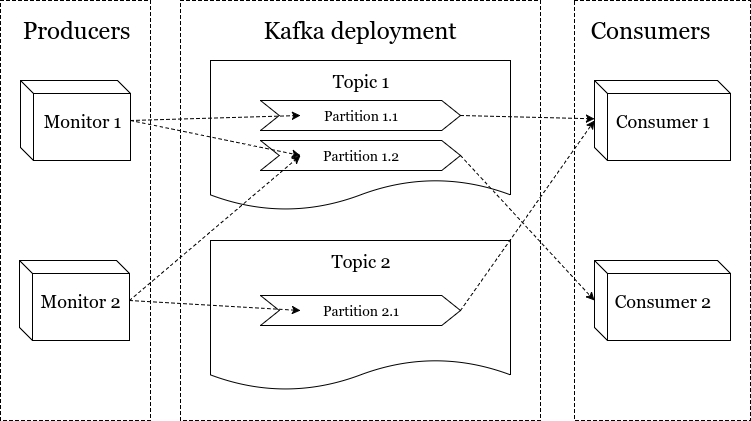
\includegraphics[width=11cm]{Figures/Figure7}
\decoRule
\caption[Exemple d'arquitectura de la comunicació amb Kafka]{Exemple d'arquitectura de la comunicació amb Kafka}
\label{fig:Kafka}
\end{figure}

En general, l'avantatge principal de Kafka i la justificació del seu ús pel nostre context és que permet una integració còmode i fiable entre diferents aplicacions que necessiten comunicar dades de forma periòdica, garantint la seva arribada. Kafka ofereix una sèrie d'APIs per configurar els \textit{producers} i \textit{consumers}, així com una configuració relativament senzilla del propi servidor. Gràcies a aquestes característiques, podem aprofitar els propis monitors per actuar com a \textit{producers} d'un \textit{stream} de dades, que es correspondrà amb les dades monitorades durant els processos d'execució, i distribuïr-les als diferents \textit{pipelines} o Kafka \textit{topics}. Així, davant possibles ampliacions i expansions d'aquest projecte, podem fàcilment incorporar components d'anàlisi gràcies al desacoblament entre la lògica interna del monitor i l'enviament i captura de dades que l'arquitectura de Kafka ens ofereix.\\

La lògica interna genèrica proposada per la implementació dels monitors serà, per tant, l'ús de l'API de \textit{producer} de Kafka per part dels monitors, pel qual cada procés de monitoratge enviarà de forma periòdica dades a un servidor Kafka específic, o Kafka \textit{endpoint}, i dins aquest desplegament, a un \textit{pipeline} o Kafka \textit{topic} específic. A la figura ~\ref{fig:Kafka} s'exposa com funciona aquesta comunicació entre els monitors i els \textit{consumers}, components que poden ser de qualsevol tipus sempre i quant implementin la lògica de \textit{consumers} pròpia e Kafka.\\

\noindent \textbf{\large Paràmetres de configuració}\\

\noindent Davant les especificacions anteriors, i per garantir el màxim nivell de personalització i configuració dels monitors, cadascun dels processos de monitoratge actius en un monitor ha de permetre definir els paràmetres relacionats amb les possibles variacions i diferències entre aquests processos, tant en temps de creació com durant la seva reconfiguració. En aquest sentit, es proposen els següents paràmetres com a genèrics per a totes les implementacions de monitors:

\begin{itemize}
\item \textbf{\textit{Time slot}}. Expressat en segons, indica la durada de cada període de monitoratge de dades (és a dir, temps que transcorre cada vegada que s'envia un nou \textit{stream} de dades).
\item \textbf{\textit{Tool name}}. Nom de l'eina (\textit{tool}) utilitzada per aquell procés de monitoratge, i que per tant implica la col·lecció d'unes dades específiques utilitzant una tècnica específica.
\item \textbf{\textit{Kafka endpoint}}. Adreça que apunta al servidor on es troba desplegat el sistema Kafka on s'han d'enviar les dades generades, ja sigui \textit{localhost} o URL pública.
\item \textbf{\textit{Kafka topic}}. Identifica el \textit{pipeline} de dades del servidor Kafka on el monitor (\textit{producer} dins el context de Kafka) ha d'enviar les dades.
\end{itemize}

És possible, tal i com veurem més endavant, que alguns monitors requereixin de paràmetres de configuració addicionals, propis del funcionament intern específic del monitor. Per aquest motiu, a banda de proporcionar una configuració bàsica pels monitors amb els paràmetres anteriors, cal permetre també una extensibilitat en quant a paràmetres de configuració.

\subsection{Disseny i arquitectura genèrica}

\begin{figure}
\centering
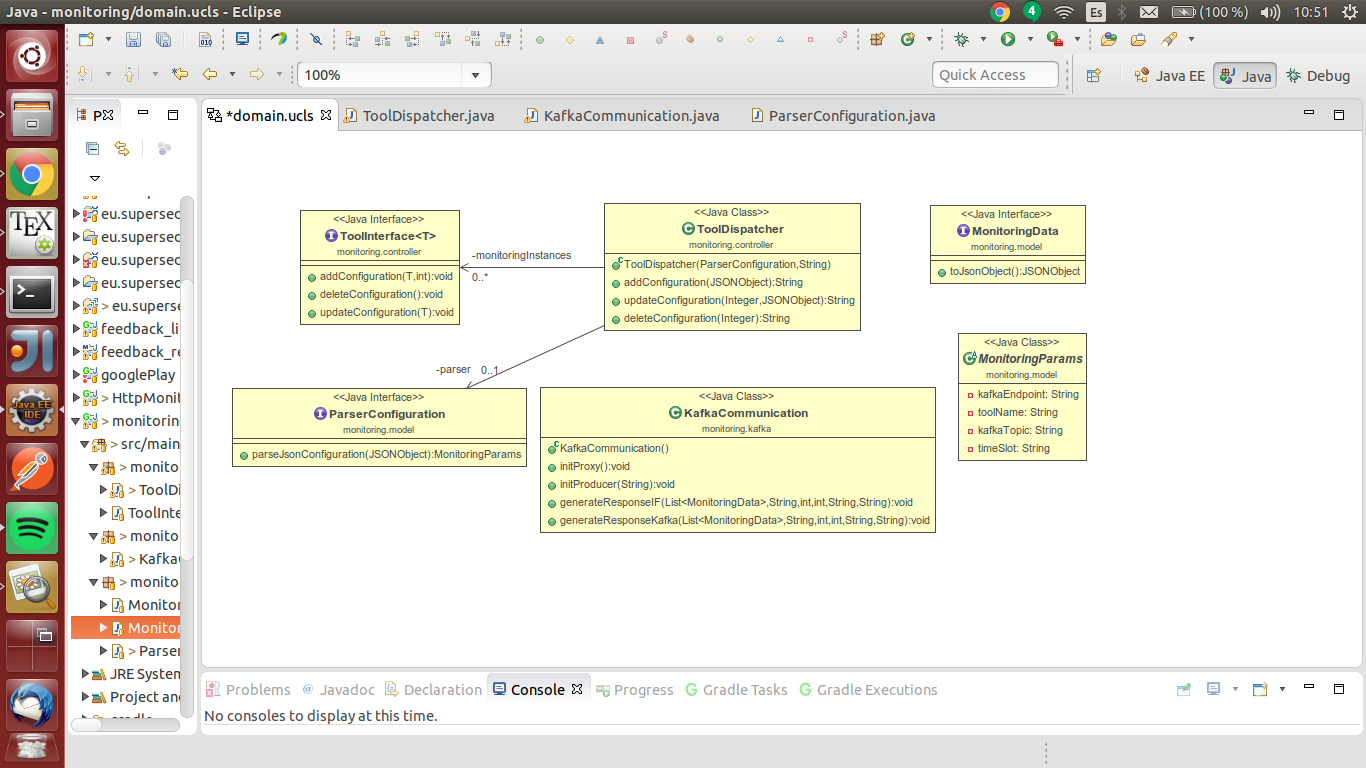
\includegraphics[width=14cm]{Figures/Figure5}
\decoRule
\caption[Arquitectura software genèrica d'un monitor]{Arquitectura software genèrica d'un monitor}
\label{fig:Figura5}
\end{figure}

Es proposa l'arquitectura definida a la figura ~\ref{fig:Figura5} a extendre per cadascuna de les implementacions de monitors. Per entendre aquesta arquitectura, a continuació s'expliquen cadascun dels elements integrats:

\begin{itemize}
\item \textbf{MonitoringParams}. Classe abstracta que cada monitor ha d'implementar que conté, de base, els paràmetres de configuració dels monitors genèrics per tots aquests. Addicionalment, cada implementació de monitor pot afegir els paràmetres i la lògica associada a aquests que consideri oportuns.
\item \textbf{ParserConfiguration}. Interfície que cada monitor ha d'implementar i que defineix un mètode per transformar un objecte JSON en una instància de la classe \textit{MonitoringParams} implementada pel propi monitor. L'objectiu és permetre així que el monitor pugui processar JSON com a format de comunicació estàndar per les peticions de configuracions, facilitant el seu ús desplegat com a servei web (especialment útil per l'Integrated Framework dins el context SUPERSEDE, tal i com s'explica al \textit{Capítol 5. Visió general del sistema}).
\item \textbf{ToolInterface}. Interfície parametritzada amb una especialització de la classe \textit{MonitoringParams} que defineix una instància de procés de monitoratge per una \textit{tool} específica. Defineix els següents mètodes:
\begin{itemize}
\item \textbf{\textit{addConfiguration(T)}} -> inicialitza el procés de monitoratge amb els paràmetres definits per la instància de T (subclasse de MonitoringParams)
\item \textbf{\textit{deleteConfiguration()}} -> atura el procés de monitoratge i elimina la instància de la \textit{tool}
\item \textbf{\textit{updateConfiguration(T)}} -> actualitza els paràmetres de configuració del procés iniciat en segon pla per la instància de la \textit{tool}
\end{itemize}
\item \textbf{ToolDispatcher}. Classe que actua com a controlador del monitor, rebent totes les peticions relacionades amb els processos de monitoratge i gestionant les diferents instàncies en execució. Defineix un \textit{ParserConfiguration} per processar la traducció de JSON (format estàndar) a \textit{MonitoringParams} pels següents mètodes:
\begin{itemize}
\item \textbf{\textit{addConfiguration(JSONObject)}} -> processa els paràmetres definits al JSONObject i inicialitza una instància de la \textit{tool} corresponent amb els paràmetres associats
\item \textbf{\textit{deleteConfiguration(int)}} -> atura el procés de monitoratge identificat per l'id proporcionat
\item \textbf{\textit{updateConfiguration(JSONObject, int)}} -> actualitza els paràmetres de configuració definits al JSONObject del procés de monitoratge identificat per int
\end{itemize}
Per tal de gestionar la \textit{tool} utilitzada en cada procés de monitoratge (que representarà una nova instància de la implementació de la interfície \textit{ToolInterface}) utilitzant el paràmetre \textit{toolName} de configuració, s'utilitza el patró \textit{reflection}. Aquest patró de disseny software es caracteritza per la modificació en temps d'execució del comportament d'un sistema; i, en el nostre cas, ens interessa per permetre  la instanciació de les diferents \textit{tools} utilitzant el seu nom sense necessitat de coneixe'l. Mitjançant l'ús del nom de la tool, i coneixent el \textit{package} on es troben implementades les tools, podem instanciar aquella tool partint únicament del nom, sense necessitat de cap altre tipus de context.
\item \textbf{MonitoringData}. Interfície que cada monitor implementa amb les dades i format que el monitor genera fruït de la seva activitat, amb la implementació d'un mètode \textit{toJsonObject()} per definir un format genèric de les dades a enviar
\item \textbf{KafkaCommunication}. Classe que implementa la comunicació amb el servidor de Kafka, i que permet enviar les dades generades per l'activitat de monitoratge. Implementa 4 mètodes segons les dues lògiques de comunicació possibles: la integrada al sistema SUPERSEDE (utilitzant \textit{proxies} de IF), i una configuració personalitzable a un Kafka endpoint específic:
\begin{itemize}
\item \textbf{\textit{initProxy()}} -> inicialitza la instància de \textit{proxy} que permet la comunicació amb el Kafka \textit{server} desplegat a IF
\item \textbf{\textit{generateResponseIF(List<MonitoringData>)}} -> envia el llistat d'instàncies de dades monitorades a través del \textit{proxy} inicialitzat
\item \textbf{\textit{initProducer(String)}} -> inicialitza un \textit{producer} de Kafka que es comunica amb l'\textit{endpoint} especificat
\item \textbf{\textit{generateResponseKafka(List<MonitoringData>)}} -> envia el llistat d'instàncies de dades monitorades a través del \textit{producer} inicialitzat
\end{itemize}
\end{itemize}

Aquesta és per tant la proposta d'una arquitectura genèrica per la implementació de cadascun dels monitors a integrar en el nostre sistema. Les especificacions tècniques tant des d'un punt de vista de requisits funcionals com requisits arquitectònics o de qualitat queden garantides, així com la seva extensibilitat d'acord amb les característiques específiques necessàries de cada monitor. La proposta genèrica s'implementa en un projecte del qual les implementacions de monitors específics han d'estendre com a subprojecte, utilitzant les funcionalitats de Gradle a tal efecte.

\subsection{Implementació de monitors}

Un cop exposada l'arquitectura i especificacions genèriques dels monitors, el següent pas és procedir a la implementació dels diferents monitors que integrarem al nostre sistema. Aquestes implementacions esdevindran possibles casos d'ús a executar, però únicament suposen exemples dins d'un ample ventall de possibilitats d'implementació.\\

En aquest projecte presentem la implementació de 3 monitors classificats en 2 tipus de monitors diferents: \textbf{monitors de xarxes socials} i \textbf{monitors de botigues d'aplicacions}. Pel primer tipus, es proposa un monitor de la xarxa social \textbf{Twitter}. Pel segon tipus, es proposen dos monitors: un monitor de \textbf{Google Play} i un altre de l'\textbf{App Store}.

\subsubsection{Twitter Monitor}

L'objectiu d'aquest monitor és supervisar i recol·lectar els tuits publicats a la xarxa social de Twitter durant un període de temps concret (definit al procés de monitoratge) que compleixen una sèrie de característiques específiques, d'acord amb els criteris que poden resultar d'interès en quant a la informació d'aquests tuits. \\

Per permetre aquesta activitat de monitoratge, i tal i com procedirem amb cadascun dels monitors, necessitem implementar com a mínim una \textit{tool} amb la qual realitzar el procés de monitoratge. Definirem una \textit{tool} anomenada \textbf{TwitterAPI} que utilitzarà \textbf{twitter4j}, una llibreria lliure no oficial de Java que permet utilitzar una arquitectura ja definida per connectar-se a les APIs de Twitter, i entre d'altres a la \textbf{Stream API}, una API que permet obrir \textit{streams} de dades per capturar i processar tots els tuits publicats en temps real que compleixin una sèrie de característiques específiques. Aquests \textit{streams} s'executaran com a \textit{threads} en segon pla i en paral·lel d'acord amb el nº de processos de monitoratge oberts.\\

Pel nostre cas, definirem dos paràmetres per filtrar els tuits monitorats: l'\textbf{autor} del tuit i l'aparició d'un \textbf{conjunt de paraules} específic al contingut del tuit. Per configurar cadascun dels processos de monitoratge d'acord a aquests dos criteris, caldrà afegir els següents paràmetres:

\begin{itemize}
\item \textbf{accounts} - llistat amb els identificadors dels autors dels quals volem obtenir els tuits 
\item \textbf{keywordExpression} - expressió booleana formada per combinacions AND, OR i NOT de diferents \textit{keywords} que el contingut del tuit ha de satisfer per ser monitorat
\end{itemize}

La \textit{Stream API} ofereix paràmetres de configuració per realitzar el \textit{tracking} dels tuits que satisfan ambdues condicions. En el cas del primer paràmetre \textit{accounts} no cal realitzar cap transformació, ja que únicament necessitem els noms únics de les comptes dels autors per obtenir els seus tuits. Contràriament, l'API únicament ofereix l'oportunitat de filtrar per combinacions de paraules expressades en la seva \textit{forma normal disjuntiva}, o \textbf{FND}. És a dir, expressions del format:\\

\centerline{\textit{$X_{1} \,\, OR \,\, X_{2} \,\, OR \,\, .. \,\, OR \,\, X_{n}$}}\bigskip

\noindent
on $X_{n}$ és una expressió booleana formada per una combinació indefinida d'operands AND:\\

\centerline{\textit{$keyword_{1} \,\, AND \,\, keyword_{2} \,\, AND \,\, .. \,\, AND \,\, keyword_{n}$}}\bigskip

Davant aquest fet, i per evitar forçar un format específic del paràmetre de configuració d'entrada, necessitem implementar una lògica interna pròpia de la \textit{tool} TwitterAPI que transformi qualsevol expressió booleana en la seva expressió FND. \\

\begin{figure}
\centering
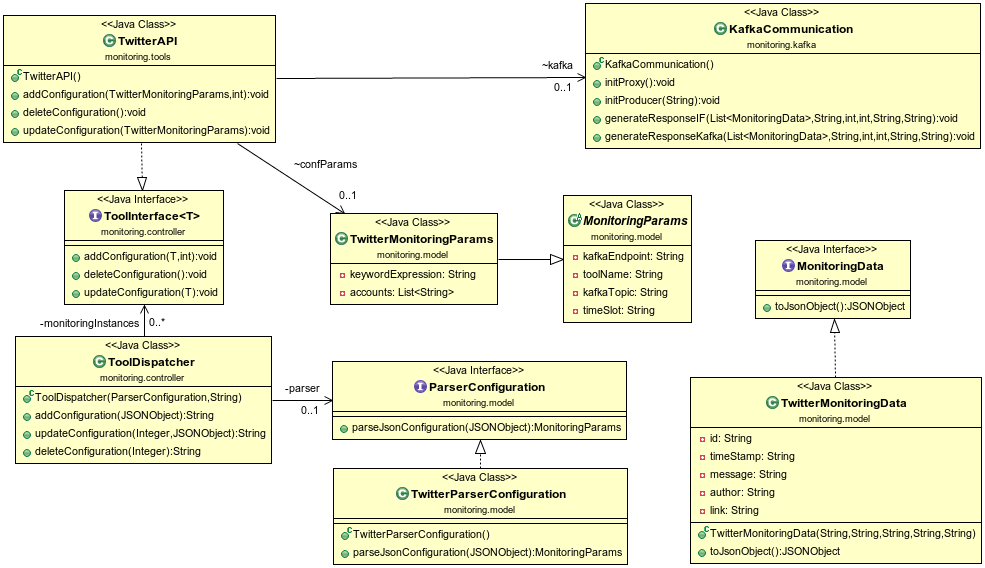
\includegraphics[width=14cm]{Figures/Figure6}
\decoRule
\caption[Arquitectura software del monitor de Twitter]{Arquitectura software del monitor de Twitter}
\label{fig:Figura6}
\end{figure}

Donats aquests detalls podem utilitzar l'arquitectura genèrica proposada anteriorment per extendre la implementació del monitor de Twitter. Aquesta arquitectura i els components implementats es troben definits a la figura ~\ref{fig:Figura6}, on podem veure aquells components reutilitzats de l'arquitectura genèrica remarcats en groc, per poder fer una comparativa ràpida sobre les classes i components que ha calgut implementar per poder definir un monitor:

\begin{itemize}
\item \textbf{TwitterMonitoringParams.} Subclasse de la classe abstracta \textit{MonitoringParams} que hereta per una banda els atributs comuns a tots els monitors (\textit{kafkaEndpoint, toolName, kafkaTopic} i \textit{timeSlot}) i per altra banda en defineix dos nous: la \textit{keywordExpression} i un llistat d'\textit{accounts}.
\item \textbf{TwitterParserConfiguration.} Implementació de la interfície que defineix la transformació del format d'entrada del monitor (JSONObject) a la instància de \textit{TwitterMonitoringParams} amb la qual el monitor (i en conseqüència la seva \textit{tool}) treballarà.
\item \textbf{TwitterMonitoringData.} Implementació de la interfície que defineix la transformació de les dades recollides durant un cicle del procés de monitoratge d'una \textit{tool} al format de sortida del monitor (JSONObject).
\item \textbf{TwitterAPI.} Implementació de la interfície que defineix la lògica de les tres operacions de qualsevol \textit{tool}: iniciar una nova configuració, modificar-ne una d'existent, i eliminar-ne una d'existent. En aquest cas disposem d'una única implementació, però tal i com veurem més endavant, l'arquitectura permet sense problema generar un conjunt de \textit{tools} diferenciades, cadascuna amb les seves característiques i dades internes, que utilitzaran les mateixes implementacions de formats de dades definides anteriorment. Aquest component serà l'encarregat d'utilitzar \textit{twitter4j} per configurar la crida a la Stream API i obrir el \textit{thread} encarregat d'anar rebent i emmagatzemant els tuits rebut. Addicionalment, serà també responsabilitat d'aquesta tool comunicar-se amb \textit{KafkaCommunication} per utilitzar el mètode de comunicació (a través de IF o personalitzat) que correspongui, d'acord amb les necessitats de la \textit{tool}.
\end{itemize}

A la figura \ref{fig:Figura12} es pot observar un exemple de l'objecte JSON generat a partir de la transformació definida per la implementació de la interfície \textit{MonitoringData}. Aquest objecte serà enviat, a través de la \textit{tool} i utilitzant la classe \textit{KafkaCommunication}, al Kafka \textit{endpoint} i Kafka \textit{topic} definits a la configuració del monitoratge. De les dades generades per la comunicació amb l'API, recollirem: \textit{idItem} (identificador del tuit), \textit{timeStamp} (moment en que s'ha realitzat el tuit), \textit{message} (contingut del mateix), \textit{author} (l'identificador de l'autor), i \textit{link} (enllaç al tuit a la plataforma Twitter). 

\begin{figure}[!h]
\centering
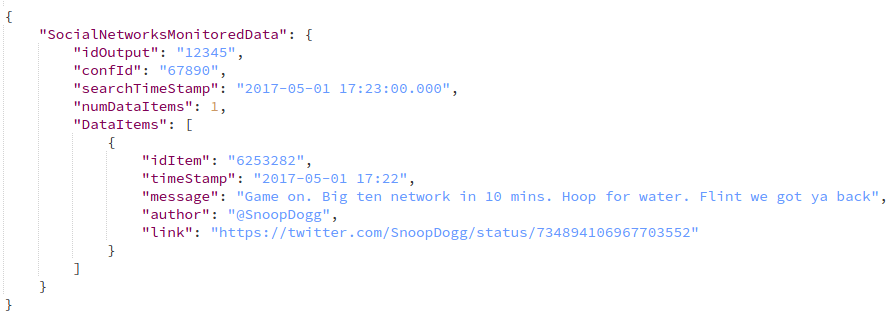
\includegraphics[width=14cm]{Figures/Figure12}
\decoRule
\caption[Exemple dades de sortida generades pel monitor de Twitter]{Exemple dades de sortida generades pel monitor de Twitter}
\label{fig:Figura12}
\end{figure}

Cal destacar que gràcies al disseny de l'arquitectura proposada anteriorment per la implementació d'un monitor integrat al nostre sistema (o, de fet, sense necessitat que l'objectiu final sigui la seva integració) ha requerit una extensió relativament senzilla. Únicament ha calgut implementar aquells aspectes propis de cada monitor, que en són 4: els paràmetres específics de configuració (1), el mapejat dels paràmetres d'entrada (2), el mapejat de les dades de sortida (3), i el funcionament de les \textit{tools} (en aquest cas, twitter4j) per realitzar els processos de monitoratge (4). D'aquesta manera satisfem un dels principals objectius: dotar al nostre sistema de la màxima extensibilitat i heterogeneïtat possible, amb la possibilitat de personalitzar l'activitat i semàntica de cada monitor partint d'una arquitectura comuna. \\

\noindent{\large{\textbf{Exposició com a servei REST}}}\\

El següent pas d'acord amb les necessitats tècniques per la integració és exposar el monitor i les seves funcionalitats com un servei web RESTful. D'aquesta manera, mitjançant la documentació d'una API per accedir a les diferents operacions d'alta, baixa i modificació d'un procés de monitoratge, podem integrar els monitors al IF del projecte SUPERSEDE i permetre així el seu accés a través de la plataforma d'integració. En aquest sentit l'ús de JSON com a format de comunicació d'entrada i sortida ens facilita la seva exposició com a servei web, que utilitzarà també el format JSON com a \textit{payload} per fer les crides. La documentació de l'API del monitor de Twitter es pot trobar a l'apèndix ~\ref{AppendixA}, on podem trobar en detall les peticions REST implementades, així com el format dels \textit{inputs} i \textit{outputs} de cadascuna de les crides.\\

Per tal de poder concebre com funcionaria la comunicació amb el monitor per iniciar una nova instància de monitoratge, la figura ~\ref{fig:Figura8} mostra un exemple d'objecte JSON utilitzat.

\begin{figure}[!h]
\centering
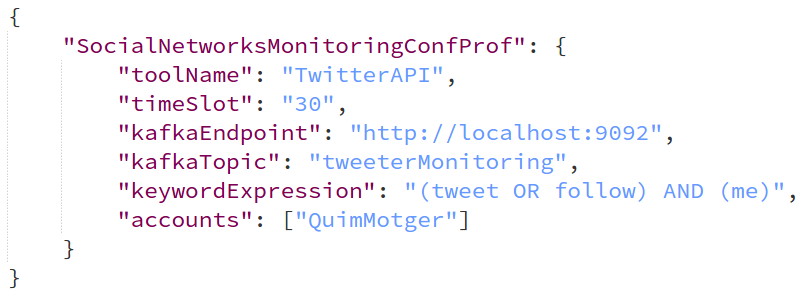
\includegraphics[width=11cm]{Figures/Figure8}
\decoRule
\caption[Exemple JSON de configuració del monitor de Twitter]{Exemple JSON de configuració del monitor de Twitter}
\label{fig:Figura8}
\end{figure}

En referència a aquesta possible petició, la figura ~\ref{fig:Figura9} mostra un exemple de la resposta (en cas d'èxit en la configuració del monitor) que retorna aquest monitor per la petició anterior. En aquesta figura, definim 2 paràmetres de retorn. Primerament,  \texttt{idConf}, que conté l'identificador de la nova instància de monitoratge creada (variable indispensable per tal que sigui usable i poder realitzar adaptacions posteriors). En segon lloc \texttt{status}, que indica si la petició s'ha realitzat amb èxit o s'ha produït algun error.

\begin{figure}[!h]
\centering
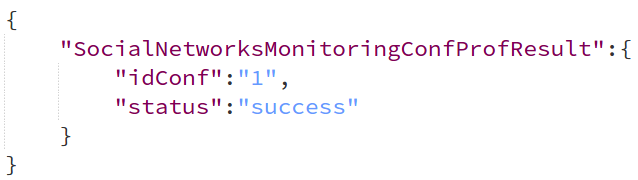
\includegraphics[width=8cm]{Figures/Figure9}
\decoRule
\caption[Exemple resposta amb èxit del monitor de Twitter]{Exemple amb èxit del monitor de Twitter}
\label{fig:Figura9}
\end{figure}

Donat el cas que s'hagi produït algun error, el format de resposta anterior no és vàlid (no s'ha creat cap instància i, per tant, cap identificador pot ser produït) ni suficient (no ens aporta informació de quin ha estat l'error). En aquest cas, un exemple de resposta seria l'exposat a la figura ~\ref{fig:Figura10}.

\begin{figure}[!h]
\centering
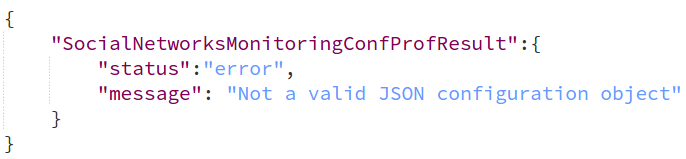
\includegraphics[width=10cm]{Figures/Figure10}
\decoRule
\caption[Exemple resposta amb error del monitor de  Twitter]{Exemple resposta amb error del monitor de Twitter}
\label{fig:Figura10}
\end{figure}

\subsubsection{Google Play Monitor}

Aquest segon monitor, encarregat del monitoratge de dades de la botiga d'aplicacions dels sistemes operatius Android, \textbf{Google Play}, pretén recollir les dades referents a les crítiques o \textit{reviews} que els usuaris de Google Play fan de les aplicacions que es descarreguen. De manera semblant al monitor de Twitter, però en un context i amb un objectiu diferent, recull dades dels usuaris i els missatges que publiquen al voltant d'un focus específic.\\

En aquest cas, i aprofitant que tenim definit un cas d'ús simple d'un monitor amb una sola \textit{tool}, podem procedir a explotar l'arquitectura dels nostres monitors i definir un monitor que utilitzi més d'una \textit{tool} per realitzar els processos de monitoratge. En aquest cas, s'ha fet una recerca a la xarxa sobre els diversos sistemes i components que existeixen (d'ús total o parcialment lliure) per realitzar el monitoratge, i s'han triat els dos següents degut a les seves característiques:

\begin{itemize}
\item \textbf{GooglePlayAPI}. \textit{Tool} que implementa una comunicació en 2n pla, similar al sistema de \textit{threads} emprat pel monitor de Twitter, amb la Google Play Developer API. Diem "similar" degut al fet que aquesta API, que funciona mitjançant un sistema d'autenticació OAuth 2.0, no permet obrir un \textit{stream} de dades com es presentava amb el monitor de Twitter, sino que permet obtenir, mitjançant crides API, les dades referents al conjunt total de \textit{reviews} publicades per una aplicació determinada en el moment de la crida. D'aquesta manera no podem obtenir un \textit{stream} de dades real de forma directa, sino que serà responsabilitat de la pròpia \textit{tool} simular aquest \textit{stream} de dades. Per fer-ho, realitzarem de forma periòdica (segons el \textit{timeSlot} definit) crides a l'API per obtenir aquestes dades, i la \textit{tool} s'encarregarà de recollir i retornar únicament les \textit{reviews} realitzades durant el període de monitoratge. Com a avantatge principal, aquesta \textit{tool} permet fer \textbf{fins a 60 crides} en 1 hora, un nombre molt elevat especialment si ho contrastem amb altres eines. Per contra, com a limitació únicament permet obtenir dades d'aplicacions de les quals l'usuari que s'ha autenticat n'és el propietari.
\item \textbf{GooglePlay-AppTweak}. Aquesta eina permet obtenir als usuaris registrats un ample ventall de dades de les aplicacions publicades a GooglePlay. En aquest cas, l'autenticació està basada en crides amb \textit{token}, i el sistema és similar a la \textit{tool} de GooglePlayAPI: necessitem simular dins el comportament de la mateixa \textit{tool} un \textit{stream} de dades parsejant els resultats de la consulta de les \textit{reviews} públiques fins al moment de la crida. En aquest cas, i en contraposició amb l'anterior \textit{tool}, com a avantatge principal aquesta eina permet \textbf{obtenir informació de qualsevol app} publicada al mercat, independentment de la seva propietat. Per contra, la seva versió gratuïta (ofereix un servei de pagament) únicament permet realitzar 100 crides al mes. Una xifra que pot resultar baixa però que, considerant la naturalesa de l'entorn monitorat, podem considerar suficient en alguns casos, ja que equivaldria a 3 crides diàries. 
\end{itemize}

La tria d'aquestes dues \textit{tools} es basa en les seves característiques d'ús i limitacions, complementàries entre elles, que ens permeten configurar un monitor prou adaptable a les necessitats del procés de monitoratge. Addicionalment a les consideracions anteriors, les dades obtingudes per ambdues \textit{tools} no són les mateixes (tot i que coincideixen en un alt percentatge), i per tal caldrà gestionar tal i com es comentarà més endavant aquesta irregularitat.\\

Per aquest cas d'ús, i degut al que hauria de ser l'escenari més habitual (monitorar en temps reals els comentaris que es realitzen sobre una aplicació específica),es defineix com a paràmetre de configuració la pròpia aplicació a monitorar, identificada pel \textbf{nom del \textit{package}}:

\begin{itemize}
\item \textbf{packageName} - identificador únic d'una aplicació publicada a Google Play
\end{itemize}

\begin{figure}
\centering
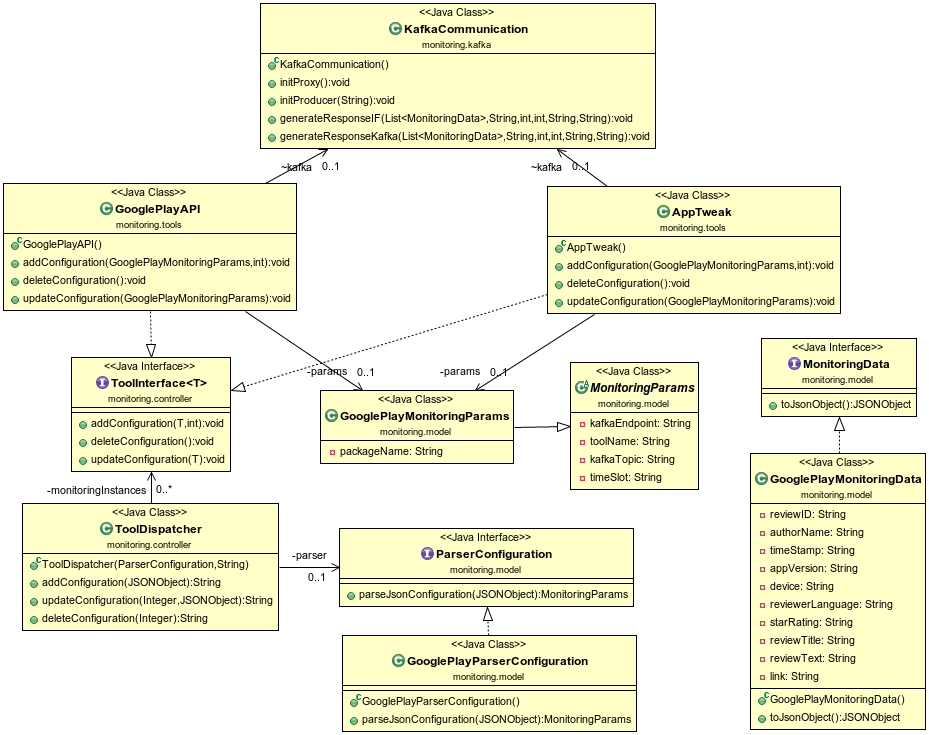
\includegraphics[width=14cm]{Figures/Figure11}
\decoRule
\caption[Arquitectura software del monitor de Google Play]{Arquitectura software del monitor de Google Play}
\label{fig:Figura11}
\end{figure}

La implementació del monitor basada en l'arquitectura genèrica definida presenta diverses similituds en comparació amb el monitor de Twitter, amb la principal diferència que, per aquest cas, tenim 2 \textit{tools} implementades a utilitzar.

\begin{itemize}
\item \textbf{GooglePlayMonitoringParams.} Subclasse de la classe abstracta \textit{MonitoringParams} que hereta els atributs comuns a tots els monitors, i afegeix com a atribut particular del monitor un string \textit{packageName}.
\item \textbf{GooglePlayParserConfiguration.} Implementació de la interfície que defineix la transformació del format d'entrada del monitor (JSONObject) a la instància de \textit{GooglePlayMonitoringParams}.
\item \textbf{GooglePlayMonitoringData.} Implementació de la interfície que defineix la transformació de les dades recollides al format JSON de sortida. En aquest cas hem d'afegir la consideració prèviament introduïda sobre la variabilitat de les dades entre les dues \textit{tools}. Davant aquest punt, podem explotar els avantatges de l'arquitectura presentada, que ens dona dues opcions:
\begin{enumerate}
\item Podem implementar una única classe que estendrà la interfície \textit{MonitoringData} i contindrà tots els paràmetres (comuns i no comuns) de les dades generades durant el procés de monitoratge. En aquest cas, la pròpia \textit{tool} crearà instàncies d'objectes monitorats amb les dades de les quals disposi, i aquelles que no pugui definir (i per tant, que prenguin valors buits o nuls) simplement no apareixeran en la transformació a objecte JSON que enviarem al Kafka \textit{endpoint}. D'aquesta manera, amb una única classe satisfem les necessitats del monitor.
\item Alternativament podem modelar un conjunt de classes que implementin la interfície, de manera que cada \textit{tool} utilitzi una d'aquestes implementacions. D'aquesta manera, disposaríem d'una implementació de \textit{MonitoringData} per cada \textit{tool} d'acord amb la informació que proporciona cadascuna d'aquestes.
\end{enumerate}
\begin{figure}[!h]
\centering
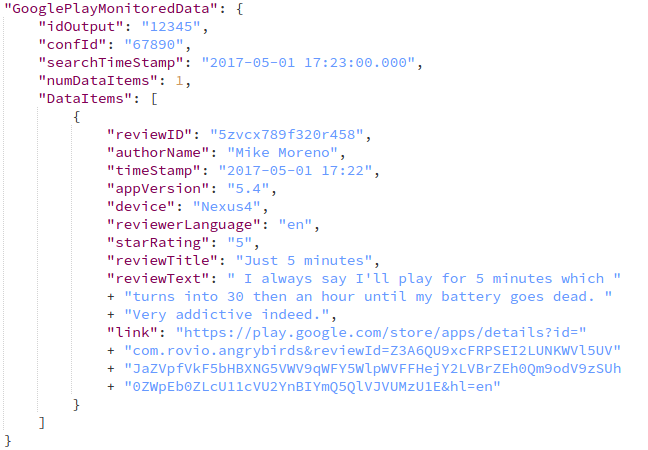
\includegraphics[width=14cm]{Figures/Figure13}
\decoRule
\caption[Exemple dades de sortida generades pel monitor de Google Play]{Exemple dades de sortida generades pel monitor de Google Play}
\label{fig:Figura13}
\end{figure}

Gràcies al disseny, cada desenvolupador podrà utilitzar l'opció que m'es s'adeqüi a les seves necessitats. La 1a opció pot resultar adequada quan p.e. el subconjunt de dades que volem obtenir sigui independent de la \textit{tool}, i per contra la 2a opció ens farà servei per desacoblar totalment les dades entre diferents tools. Pel nostre cas d'ús, considerarem la 1a opció, ja que dins la integració de SUPERSEDE, l'anàlisi d'aquestes dades serà independent de la \textit{tool} utilitzada.
\item \textbf{GooglePlayAPI}. Implementació de \textit{ToolInterface} que utilitza l'API de Google Play Developer. Aquesta \textit{tool} implementa una comunicació mitjançant autenticació OAuth 2.0 mitjançant els \textit{tokens} obtinguts al registrar un usuari de Google Play com a \textit{developer}. Per aquest projecte s'ha utilitzat un compte personal de Google Play compartit amb altres estudiants del Grau en Enginyeria Informàtica, per tal de poder probar i validar aquesta \textit{tool} (ja que, tal i com especificat anteriorment, únicament ens permet obtenir dades de les aplicacions de les quals l'usuari n'és l'autor). Degut al gran volum de dades que es poden generar al demanar les \textit{reviews} d'una aplicació, l'API funciona mitjançant un sistema de paginació. És a dir: la crida REST per obtenir les reviews retorna un subconjunt de mida relativament petita i, addicionalment, un \textit{token} que permet referenciar el següent subconjunt (o pàgina) de reviews. Aquest token s'utilitza per realitzar una nova crida, que conté un nou subconjunt de reviews i, addicionalment, un nou \textit{token} per la següent pàgina. D'aquesta manera, les dades venen paginades i subdividides. És responsabilitat de la \textit{tool} implementar la lògica per realitzar les crides de forma iterativa. 
Aquest tractament pot ser un procés relativament lent (en termes computacionals). Però això no suposa un trencament amb la filosofia de "fotografiar" el sistema en un moment determinat: en el moment que es fa la crida REST, l'API captura les \textit{públiques} en aquell moment, i construeix els objectes de dades paginats, de tal manera que encara que es triguin uns segons en computar totes les pàgines de dades, aquestes sempre seran una representació del moment en que s'ha fet la primera crida, corresponent al final d'un cicle de monitoratge de durada definida al \textit{timeSlot.}
\item \textbf{AppTweak}. Implementació de \textit{ToolInterface} que utilitza l'API de AppTweak. A diferència de l'anterior, tant l'autenticació com la lògica per obtenir les dades és molt més senzilla. En el cas de la primera, funciona mitjançant l'ús d'un \textit{token} a la capçalera de la crida REST, únic per usuari a la plataforma. En el cas de la segona, una sola crida REST retorna totes les dades corresponents a les \textit{reviews} d'aquella aplicació.
\end{itemize}

\noindent{\large{\textbf{Exposició com a servei REST}}}\\

De forma anàloga a l'exposició com a servei del monitor de Twitter, cal dissenyar i implementar un servei REST per desplegar les funcionalitats del monitor de Google Play. La figura ~\ref{fig:Figura14} mostra un exemple d'un possible objecte JSON de configuració del monitor.\\

\begin{figure}[!h]
\centering
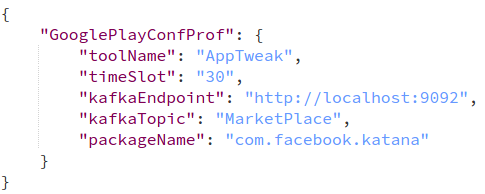
\includegraphics[width=11cm]{Figures/Figure14}
\decoRule
\caption[Exemple JSON de configuració del monitor de GooglePlay]{Exemple JSON de configuració del monitor de GooglePlay}
\label{fig:Figura14}
\end{figure}

Tot i que el paràmetre de \textit{toolName} ja l'havíem vist en l'anterior monitor, ja que és necessari per la instanciació de la \textit{tool} utilitzant el patró reflexió, en aquest cas cobra una especial importància, ja que al disposar d'un conjunt de \textit{tools} podem utilitzar els noms d'aquestes per configurar el monitor; en aquest cas, amb les \textit{tools} de \textbf{GooglePlay} i \textbf{AppTweak}.\\

\subsubsection{App Store Monitor}

\section{Monitor Manager}

Partint de l'arquitectura genèrica dels monitors, i l'exemplificació d'aquesta en casos d'ús reals (i per tant a seva implementació), disposem dels primers components essencials per construïr el nostre sistema. En aquest punt disposem d'un subconjunt de monitors que satisfan les seves especificacions tècniques individuals, relacionades amb l'activitat de monitoratge. Però necessitem anar un pas mes enllà en l'evolució del nostre sistema per satisfer els objectius generals d'adaptabilitat, i procedir a desenvolupar components d'integració.\\

Per aquest objectiu, el primer pas és el desenvolupament del \textbf{Monitor Manager}. Aquest component, tal com el seu nom indica (i com s'ha presentat al \textit{Capítol 5. Visió general del sistema}), s'encarrega de la gestió de tots els monitors desplegats al sistema. Per gestió entenem la satisfacció dels següents requisits funcionals:

\begin{enumerate}
\item \textbf{Inicialització de procés de monitoratge per a un monitor específic.} El component ha de ser capaç de rebre una petició d'inicialització de procés de monitoratge per un dels monitors integrats al sistema, i redireccionar aquesta petició al monitor corresponent, de manera que aquest pugui processar i executar la petició.
\item \textbf{Modificació de procés de monitoratge per a un monitor específic.} Donat un procés de monitoratge existent per a un monitor específic integrat al sistema, el component ha de rebre una petició de reconfiguració d'aquest, processar-la i redireccionar-la al monitor corresponent.
\item \textbf{Aturada de procés de monitoratge per a un monitor específic.} Donat un procés de monitoratge existent per a un monitor específic integrat al sistema, el component ha de rebre una petició per aturar-lo, processar-la i redireccionar-la al monitor corresponent.
\end{enumerate}

Com es pot extreure de les funcionalitats anteriors, l'objectiu principal d'aquest component és \textbf{processar} i \textbf{redireccionar} les peticions relacionades amb accions sobre els monitors desplegats. D'aquesta manera, i enfocat al màxim nivell d'independència entre components, estem afegint un nivell d'abstracció per sobre dels monitors que permetrà la comunicació amb la resta de components del sistema sense necessitat de conèixer els detalls semàntics i tècnics de cada implementació dels monitors.\\

Per tant, com a part de la tasca en el disseny i desenvolupament d'aquest monitor, caldrà definir un punt d'entrada únic pels 3 tipus d'operacions: \textbf{iniciar}, \textbf{modificar} i \textbf{aturar} un procés de monitoratge en un monitor específic. La lògica interna del Monitor Manager, per tant, s'haurà d'encarregar de processar aquestes peticions, identificar a quin monitor pertoca, i redireccionar-la al mateix.

\subsection{Especificacions tècniques i funcionals}

Les especificacions tècniques en les que ens basarem per dissenyar i implementar el Monitor Manager requereixen satisfer una \textbf{integració} que actuï com a pont \textbf{únic} entre components tercers del sistema i els nostres monitors. Seguint els criteris presentats anteriorment, caldrà considerar els següents punts:

\begin{enumerate}
\item \textbf{INPUT - Petició de configuració de monitor}. Descripció dels paràmetres i el format genèric d'aquests per realitzar la redirecció de la petició.
\item \textbf{\textit{ACTION} - Processat de la petició}. Tractament del format genèric dels paràmetres i interpretació d'acord amb el monitor adreçat.
\item \textbf{\textit{OUTPUT} - Redirecció al monitor}. Enviament de la petició processada cap al monitor.
\end{enumerate}

\noindent \textbf{\large Petició de configuració de monitor}\\

\noindent La petició de configuració s'ha de rebre en un format genèric que el propi Monitor Manager sigui capaç d'encapsular, identificar el monitor al qual cal enviar-la, i redireccionar-la posteriorment. Per fer-ho, independentment del format, necessitem identificar dos factors claus que el Monitor Manager ha de rebre:

\begin{itemize}
\item El \textbf{monitor específic} al qual s'ha de redireccionar la petició
\item Els \textbf{paràmetres de configuració} per aquell monitor: \textit{toolName} + \textit{kafkaEndpoint} + \textit{kafkaTopic} + \textit{timeSlot} + [paràmetres específics]
\end{itemize} 

Respecte al 2n punt, es tracta d'informació formatada que el monitor específic necessita, i que per tant podem reaprofitar i mantenir estructurada tal i com s'ha documentat prèviament. Respecte al 1r punt, en canvi, es tracta d'informació que el Monitor Manager necessita addicionalment per processar la redirecció.\\

En aquest punt cal decidir si aquesta informació l'afegim de forma implícita a l'objecte JSON de configuració, o bé si busquem una alternativa que ens permeti mantenir l'objecte JSON intacte. En el primer cas, la informació relativa a la configuració queda totalment integrada en un sol objecte JSON que utilitzarem per \textbf{redireccionar} i \textbf{configurar} el monitor. Però això obliga a modificar el format d'aquest JSON, afegint informació addicional que el monitor no necessita. En el segon cas, en canvi, podem mantenir un objecte de configuració que es propaga entre els diferents components: primer com a \textit{input} del Monitor Manager, i després com a \textit{output} redireccionat com a \textit{input} al monitor específic. Alternativament, però, cal buscar una forma de comunicar al Monitor manager a quin monitor trobarà la \textit{tool} sobre la qual hem d'iniciar un procés de monitoratge.\\

\begin{figure}[!h]
\centering
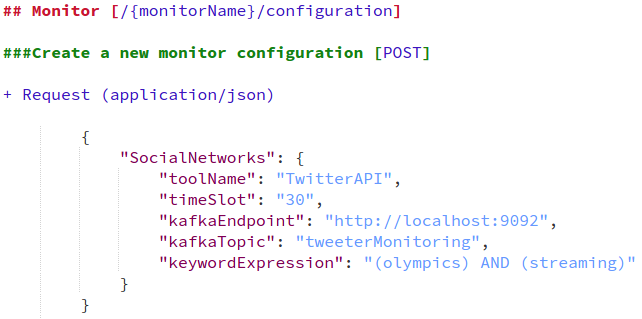
\includegraphics[width=11cm]{Figures/Figure15}
\decoRule
\caption[Exemple JSON de configuració de monitor al Monitor Manager]{Exemple JSON de configuració de monitor al Monitor Manager}
\label{fig:Figura15}
\end{figure}

En aquest sentit aprofitarem la necessitat d'exposició dels components com a serveis RESTful per, mitjançant el propi disseny de la API que implementarà el Monitor Manager, definir aquest paràmetre. En el  disseny d'aquesta API, present a l'apèndix ~\ref{AppendixA}, proposem com a paràmetre dins la URL de les 3 crides a implementar (creació, modificació i eliminació) el propi identificador del monitor. Així, exemplificant la crida per crear una configuració sobre el monitor de Twitter, podem veure a la figura ~\ref{fig:Figura15} la URL que defineix el recurs per realitzar aquesta operació (on \textit{monitorName} és el paràmetre de la URL que identifica el monitor a redireccionar), així com un exemple de JSON que rebrà. Com es pot apreciar, aquest presenta els mateixos camps que el JSON definit als monitors.\\

Amb aquestes dades d'entrada, el Monitor Manager ja és capaç de realitzar la redirecció al monitor corresponent.\\

\noindent \textbf{\large Processat de la petició}\\

\noindent Un cop definida la informació i el seu format d'entrada necessaris per satisfer les especificacions tècniques, cal avaluar com partim d'aquesta informació a la petició de configuració de monitors.\\

Ja que la única tasca a realitzar és la redirecció (ja que les dades no cal que siguin tractades), hem de partir del paràmetre \textit{monitorName} per identificar el monitor al qual redireccionar. El component IF exposa, de manera separada, la implementació de classes o \textit{proxies} diferents per cada monitor implementat. És a dir: per cada monitor que vulguem integrar i registrar al nostre sistema, necessitarem afegir-ho a IF per garantir-ne la integració de la comunicació, mitjançant la implementació d'un \textit{proxy} amb els mètodes de comunicació que ofereix. Per tant, la responsabilitat del Monitor Manager serà utilitzar el paràmetre \textit{monitorName} per discernir entre els \textit{proxies} implementats per IF i seleccionar aquell que es correspongui al monitor al qual la petició ha d'anar adreçada. \\

\noindent \textbf{\large Redirecció al monitor}\\

\noindent Finalment, identificat i instanciat el \textit{proxy} el Monitor Manager executarà una crida \textit{addConfiguration}, \textit{updateConfiguration} o \textit{deleteConfiguration} en funció de l'operació enviada. De nou en aquest sentit s'aprofita l'\textit{input} d'aquest component mitjançant la seva exposició com a servei: cada mètode de creació, modificació i eliminació crida al mètode corresponent del \textit{proxy} definit per \textit{monitorName}. A aquest \textit{proxy} s'enviarà la instància de configuració rebuda d'entrada, reaprofitant exactament el mateix format, mantenint així la uniformitat de les dades desitjada.

\subsection{Disseny i implementació}

En definitiva, d'acord amb les necessitats establertes, la implementació del Monitor Manager es basarà simplement en el disseny i implementació d'un servei REST que implementi els 3 mètodes definits anteriorment, i que la seva lògica interna s'encarregui simplement d'identificar, a partir del nom del monitor rebut com a paràmetre, el \textit{proxy} que implementa la comunicació amb aquell monitor. A la figura ~\ref{fig:monitor-manager} podem veure la interfície que defineix els 3 mètodes que exposen les 3 funcionalitats bàsiques se les configuracions de monitors. A partir d'aquesta interfície, només caldrà exposar-lo com a servei web RESTful per la seva integració a IF.\\

\begin{figure}[!h]
\centering
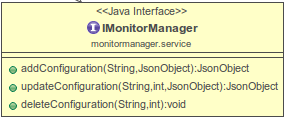
\includegraphics[width=8cm]{Figures/monitor-manager-interface}
\decoRule
\caption{Disseny de la interfície del Monitor Manager}
\label{fig:monitor-manager}
\end{figure}

Cal notar que un dels paràmetres que reben com a paràmetre les 3 peticions ha de ser el nom del monitor al qual va redirigit aquesta petició. 

\section{Orchestrator}

Aquest component forma part de la integració d'aquest projecte dins el projecte SUPERSEDE, i per tant el disseny i desenvolupament d'aquest ha estat únicament realitzat com a part d'aquest TFG de forma parcial. Concretament, aquelles parts referents a l'activitat de monitoratge i reconfiguració de monitors.\\

La seva tasca principal és actuar de pont entre els components encarregats d'aplicar adaptacions (\textit{Enactments}) i aquells encarregats del monitoratge (\textit{Monitoring}), que recordem forma part del cicle MAPE-k descrit anteriorment. Aquest és necessari en el moment que diversos sistemes d'adaptabilitat apliquen modificacions en diversos sistemes encarregats de monitorar dades. Aquest TFG n'és un cas específic. Si, per contra, aquest hagués d'actuar com a sistema independent, l'abstracció garantida pel Monitor Manager, que unifica tots els monitors sota un únic punt d'entrada, ja seria suficient per facilitar la comunicació, el manteniment i l'extensió de components. Per contra, si haguéssim volgut afegir la lògica del Monitor Manager al mateix Orchestrator, i aprofitar la seva necessitat dins SUPERSEDE per estalviar-nos una capa en el sistema, ens veuríem obligats a aplicar modificacions i manteniment a l'Orchestrator, un component genèric d'integració, davant modificacions específiques pel nostre cas d'ús. Per tal d'evitar això, s'ha decidit mantenir aquests dos components per separat, i garantir un desacoblament de components el més alt possible.\\

Addicionalment, a aquest component se li assigna una responsabilitat superior associada a la gestió i control del sistema de monitoratge i les seves especificacions. Amb això es fa referència a la persistència i control de metadades relacionades amb els monitors, que ens permeten tenir de forma integrada coneixement sobre el nostre sistema. Aspectes com, p.e., els \textbf{tipus de monitors} integrats, que engloben un conjunt de monitors treballant sobre una mateixa àrea, o bé les \textbf{tools implementades} per cada tipus de monitor.\\

\subsection{Especificacions tècniques i funcionals}

En general, per tant, podem concebre l'Orchestrator com un \textbf{component d'integració} i un \textbf{repositori de metadades}. Per tant, independentment de les funcionalitats que caldrà implementar (que a continuació detallarem), caldrà tenir en compte dues característiques bàsiques:

\begin{itemize}
\item Haurà de gestionar la \textbf{persistència} de dades relacionades amb els monitors, i per tant caldrà afrontar el \textbf{disseny} i la \textbf{implementació} d'una base de dades.
\item Paral·lelament, caldrà implementar un controlador exposat com a \textbf{servei REST} que exposi les seves funcionalitats i, addicionalment, permeti la seva integració a IF.
\end{itemize}

Per definir els detalls d'aquestes dues branques, necessitem primer definir amb quines metadades estarem treballant i com estructurarem el seu contingut. Definirem, essencialment, tres entitats principals:

\begin{enumerate}
\item \textbf{Monitor configuration}. Instància ja definida anteriorment, que representa l'execució d'una \textit{tool} amb uns paràmetres de configuració específics.
\item \textbf{Monitor tool}. Engloba les metadades associades a aquella \textit{tool} i té associades totes les configuracions en procés d'execució. D'aquesta manera, les dades referents a les configuracions actives per a una \textit{tool} no es troben exclusivament al desplegament del propi monitor, el que suposaria la necessitat d'accedir al propi monitor. Contràriament, aquestes dades es trobaran integrades a l'Orchestrator, el que facilitarà la seva gestió quan es tracti de casos exclusivament de lectura de dades. Aquest darrer propòsit, en qualsevol cas, no entra part del context d'aquest projecte, sinó que està orientat a la integració del TFG amb SUPERSEDE i l'explotació d'aquestes dades.
\item \textbf{Monitor type}. Engloba un conjunt de \textit{tools} que pertanyen a monitors d'una mateixa categoria, com per exemple \textit{Social Networks} o \textit{Market Places}. Aquest agrupament per tipus, com en el cas anterior, tampoc és rellevant pel nostre context, però ens ofereix integració de dades que resulta d'interès en termes analítics.
\end{enumerate}

% Please add the following required packages to your document preamble:
% \usepackage{multirow}
\begin{table}[htb]
\centering
\label{InstanciacioOrchestrator}
\begin{tabular}{|l|l|l|}
\hline
\textbf{Monitor Type}            & \textbf{Monitor Tool}          & \textbf{Monitor configuration} \\ \hline
\multirow{3}{*}{Social Networks} & \multirow{3}{*}{TwitterAPI}    & TwitterAPI-Conf1               \\ \cline{3-3} 
                                 &                                & TwitterAPI-Conf2               \\ \cline{3-3} 
                                 &                                & TwitterAPI-Conf3               \\ \hline
\multirow{6}{*}{Market Places}   & \multirow{2}{*}{GooglePlayAPI} & GooglePlay-Conf1               \\ \cline{3-3} 
                                 &                                & GooglePlay-Conf2               \\ \cline{2-3} 
                                 & GooglePlay-AppTweak            & GooglePlay-AppTweak-Conf1      \\ \cline{2-3} 
                                 & \multirow{2}{*}{iTunesApple}   & iTunesApple-Conf1              \\ \cline{3-3} 
                                 &                                & iTunesApple-Conf2              \\ \cline{2-3} 
                                 & AppStore-AppTweak              & AppStore-AppTweak-Conf1        \\ \hline
\end{tabular}
\caption{Exemple d'instanciació del sistema de monitoratge}
\end{table}

Per tal d'entendre bé aquest esquema, podem visualitzar un esquema conceptual a la taula 7.1 que presenta un exemple de constitució d'un sistema de monitoratge en actiu com el que hem anat descrivint al llarg d'aquest projecte. Bàsicament tenim dos tipus de monitors, \textbf{Social Networks} i \textbf{Market Places}. Pel primer tenim definida una única \textit{tool}, \textbf{TwitterAPI}; pel segon, tenim definides 4, dues per cada \textit{market place} (\textit{AppStore} i \textit{GooglePlay}). Fixem-nos en el detall que en cap moment estem contemplant l'entitat \textbf{monitor} en aquest esquema. Això es deu al fet que, dins el nostre esquema, l'entitat monitor només és significativa des d'un punt de vista físic, com a punt integrat de desplegament que agrupa un conjunt de \textit{tools}. Podríem considerar que existeixen punts comuns entre \textit{tools} dins un mateix monitor, com p.e. la implementació dels paràmetres d'entrada o de sortida. Però la nostra arquitectura no restringeix aquest aspecte. Dins un mateix monitor, cada \textit{tool} pot implementar aquestes interfícies i classes d'acord amb les seves necessitats. D'aquesta manera, el concepte monitor únicament és significatiu des del punt de vista d'implementació i desplegament físic, no lògic o de metadades. Per tant, no considerarem aquesta entitat dins el nostre esquema conceptual.\\

Finalment, a la taula podem veure un conjunt d'exemple de configuracions. Aquest no vindrà limitat per cap restricció, i tot i que cada monitor s'ha d'encarregar en última instància de gestionar-ho, serà a través del Orchestrator i el Monitor Manager que es gestionaran les altes, baixes i modificacions d'aquests.\\

\noindent \textbf{\large Peticions de configuració del sistema de monitoratge}\\

\noindent Mitjançant l'exposició de les funcionalitats com a servei REST, l'Orchestrator haurà de rebre el conjunt de peticions amb dos objectius principals: la \textbf{gestió de metadades} del nostre sistema de monitoratge, i la \textbf{redirecció de les peticions} associades directament a configuracions del sistema. La definició d'aquests mètodes d'entrada no ve a ser més que el disseny d'un controlador basat en les operacions \textbf{CRUD} (\textit{\textbf{C}reate}, \textit{\textbf{R}ead}, \textit{\textbf{U}pdate}, \textit{\textbf{D}elete}) per les entitats \textit{Monitor Type}, \textit{Monitor Tool} i \textit{Monitor Configuration}. A la taula 7.2 podem visualitzar un resum conceptual dels mètodes que necessitarem definir, i quins paràmetres caldrà definir per cadascun d'ells.\\

\begin{table}[htb]
\centering
\label{PeticionsOrchestrator}
\begin{tabular}{|p{4cm}|p{6cm}|p{3cm}|}
\hline
\textbf{Operació}                            & \textbf{Definició}                                                        & \textbf{Paràmetres}                                                                                                           \\ \hline
\multicolumn{3}{|c|}{\textbf{Monitor Type}}                                                                                                                                                                                                                        \\ \hline
Llistat de Monitor Types                     & Retorna el llistat de tots els Monitor Types instanciats al sistema       & /                                                                                                                                       \\ \hline
Obté un Monitor Type                         & Retorna les dades d'un Monitor Type específic                             & - nomTipus                                                                                                                              \\ \hline
Alta de Monitor Type                         & Crea una nova instància de Monitor Type                                   & - nomTipus                                                                                                                              \\ \hline
Baixa de Monitor Type                        & Elimina una instància de Monitor Type existent                            & - nomTipus                                                                                                                              \\ \hline
\multicolumn{3}{|c|}{\textbf{Monitor Tool}}                                                                                                                                                                                                                        \\ \hline
Llistat de Tools per Monitor Type            & Retorna el llistat de totes les Tools implementades per a un Monitor Type & - nomTipus                                                                                                                              \\ \hline
Obté una Tool per un Monitor Type            & Retorna les dades d'una Tool per un Monitor Type                          & \begin{tabular}[c]{@{}l@{}}- nomTipus\\ - nomTool\end{tabular}                                                                          \\ \hline
Alta de Tool per un Monitor Type             & Crea una nova Tool per un Monitor Type                                    & \begin{tabular}[c]{@{}l@{}}- nomTipus\\ - nomTool\\ - nomMonitor\end{tabular}                                                           \\ \hline
Baixa de Tool per un Monitor Type            & Elimina una Tool existent per un Monitor Type                             & \begin{tabular}[c]{@{}l@{}}- nomTipus\\ - nomTool\end{tabular}                                                                          \\ \hline
\multicolumn{3}{|c|}{\textbf{Monitor Configuration}}                                                                                                                                                                                                               \\ \hline
Llistat de Configurations per una Tool       & Retorna el llistat de totes les Configurations actives per una Tool       & \begin{tabular}[c]{@{}l@{}}- nomTipus\\ - nomTool\end{tabular}                                                                          \\ \hline
Obté una Configuration per una Tool          & Retorna les dades d'una Configuration per una Monitor Tool                & \begin{tabular}[c]{@{}l@{}}- nomTipus\\ - nomTool\\ - idConf\end{tabular}                                                               \\ \hline
Alta de Configuration per una Tool           & Crea una nova Configuration per una Monitor Tool                          & \begin{tabular}[c]{@{}l@{}}- nomTipus\\ - nomTool\\ - timeSlot\\ - kafkaEndpoint\\ - kafkaTopic\\ - {[}custom{]}\end{tabular} \\ \hline
Modificació d'una Configuration per una Tool & Modifica els paràmetres d'una Configuration existent per una Monitor Tool & \begin{tabular}[c]{@{}l@{}}- nomTipus\\ - nomTool\\ - idConf\\ - timeSlot\\ - kafkaEndpoint\\ - kafkaTopic\\ - {[}custom{]}\end{tabular} \\ \hline                                                                                                                    
Baixa d'una Configuration per una Tool       & Elimina una Configuration existent per una Monitor Tool                   & \begin{tabular}[c]{@{}l@{}}- nomTipus\\ - nomTool\\ - idConf\\ - timeSlot\\ - kafkaEndpoint\\ - kafkaTopic\\ - {[}custom{]}\end{tabular} \\ \hline
\end{tabular}
\caption{Llistat de peticions d'entrada del Orchestrator}
\end{table}

Respecte aquests mètodes, cal considerar els identificadors de cadascuna d'aquestes entitats:

\begin{itemize}
\item \textbf{Monitor Type}. S'identifica per un \textbf{nom} únic
\item \textbf{Monitor Tool}. S'identifica per un \textit{Monitor Type} (un nom de \textit{Monitor Type}) + un \textbf{nom} únic de tool
\item \textbf{Monitor Configuration}. S'identifica per un \textit{Monitor Type} (un nom de \textit{Monitor Type}) + una \textit{Monitor tool} (un nom de \textit{Monitor Tool}) + un \textbf{id} únic de la configuració
\end{itemize}

En general, tota la informació d'entrada que necessita per executar cadascuna de les operacions es basa en identificar el recurs sobre el qual aplicar l'acció. Aquesta identificació a nivell de configuració, que és la darrera entitat que a nosaltres ens interessa considerar, es basa en un triplet de la forma:\\

\centerline{\textbf{monitorType + monitorTool + idConf}}\bigskip

Només en un cas necessitem afegir més informació, que serà pels dos casos a treballar en aquest projecte: la \textbf{creació d'una configuració} i la seva \textbf{reconfiguració} (o actualització). En aquest cas, i tal i com s'ha definit en l'especificació i disseny dels monitors, caldrà afegir d'una banda aquells paràmetres obligatoris per a tot monitor, i addicionalment aquells propis de cada \textit{tool}.\\

\noindent \textbf{\large Actualització de metadades}\\

\noindent El comportament intern de l'Orchestrator serà relativament senzill, ja que únicament necessita contemplar l'actualització de metadades i el processament de les peticions realitzades per redirigir-les, si s'escau, al monitor corresponent.\\

Considerant primer \textbf{l'actualització de metadades}, l'Orchestrator actualitzarà d'acord a l'operació executada modificacions a la base de dades d'acord amb \textbf{creació}, \textbf{actualització} i eliminació de les entitats prèviament definides. En cas que es tracti d'operacions de lectura, només caldrà accedir a la base de dades i llegir les dades associades a la petició realitzada. Aquest aspecte de l'acció interna el considerarem trivial, ja que es tracta únicament de modificacions associades a una BDD relacional (veure més endavant a \textit{Implementació del Orchestrator}), i no resulta d'especial interès per la finalitat del nostre projecte.\\

\noindent \textbf{\large Redirecció de peticions}\\

\noindent Per altra banda cal definir la \textbf{redirecció de peticions} a monitors. Fixem-nos que, al disposar de totes les dades integrades, aquesta únicament caldrà contemplar-la pels casos en els que no només cal realitzar modificacions sobre les pròpies metadades (o bé simplement realitzar lectures), sinó també realitzar canvis relacionats amb l'execució real dels monitors. Això per tant inclourà: \textbf{alta} de configuració, \textbf{reconfiguració} d'una configuració, i \textbf{eliminació} d'una configuració. En aquests 3 casos, l'Orchestrator haurà de realitzar la redirecció amb el Monitor Manager, utilitzant la integració amb IF.\\

El mateix problema de criteri de redirecció sorgeix que en el cas del Monitor Manager. Necessitem saber quina \textit{tool} va associada a quin monitor, per tal d'indicar al Monitor Manager a quin monitor es troba implementada aquella \textit{tool}. El Monitor Manager requeria aquest paràmetre en la petició, ja que ell no té constància d'aquestes dades. Però a l'Orchestrator sí que disposem d'aquesta metadada, associada a una \textit{tool}, i definida en el moment de creació, tal i com observem també a la taula 7.2. Per tant, a l'hora d'instanciar el \textit{proxy} de IF per comunicar-se amb el Monitor Manager, cridarem al mètode corresponent al Monitor identificat per aquest atribut. D'aquesta manera la redirecció queda satisfeta.\\

\subsection{Disseny i implementació}

Sense entrar en molt detall en els aspectes d'implementació de les especificacions prèviament descrites, podem trobar els detalls d'aquesta a: 

\begin{itemize}
\item Disseny dels controladors de domini, definits a la figura ~\ref{fig:orchestrator}
\item Disseny de l'esquema de la \textbf{base de dades}, definit a l'apèndix ~\ref{AppendixA}
\item Disseny de l\textbf{API RESTful}, definit a l'apèndix ~\ref{AppendixA}
\end{itemize}

Degut a que el comportament i els detalls específics no són d'especial interés pel domini d'aquest projecte, no s'entrarà amb més detall en la informació referent a la implementació tècnica, que s'ha realitzat seguint les instruccions i els requisits tècnics específics del component Orchestrator genèric implementat per \textit{partners} del projecte SUPERSEDE.

\begin{figure}[!h]
\centering
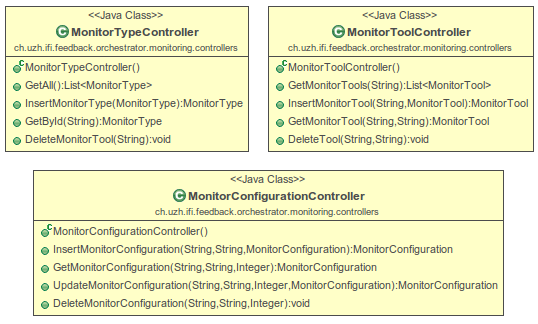
\includegraphics[width=14cm]{Figures/orchestrator}
\decoRule
\caption{Disseny dels controladors de l'Orchestrator}
\label{fig:orchestrator}
\end{figure}